\chapter{长时间目标跟踪算法}
\hspace*{0.85cm}自动目标搜索与跟踪系统需要具备对感兴趣目标进行长时间跟踪的能力。长时间目标跟踪器需要满足以下两个条件:(1)当目标跟丢后,能够重新进行初始化,矫正跟踪误差;(2)当目标暂时离开视野范围,并再次进入视野时,能够再次跟踪。
现有的基于在线学习(online-learning)的目标跟踪器都不能胜任长时间跟踪的任务,因为在线学习的方式存在``漂移''(drift)问题,一旦跟丢,很难重新初始化。另一方面,在跟踪过程中目标的外观和形状可能会随时发生改变,为了适应目标的动态变化,在线学习机制又是必不可少的。因此,为了实现长时间的目标跟踪,离线的先验知识和在线学习机制都是不可或缺的。第\ref{chap:2}章中实现的基于深度学习的目标检测算法经过大量图像数据的训练,能够在给定图像上可靠地检测感兴趣目标,可以作为目标离线的先验知识来完成目标的初始定位以及跟丢后的重定位。现有的在线式跟踪算法(Struck \cite{struck},KCF \cite{kcf} 等)用来适应目标的动态变化。本文采用一种离线--在线式的方式来实现长时间的目标跟踪,其中基于深度学习的离线知识是目标跟踪系统得以长时间运行的基石。离线的先验知识于在线学习的过程通过大名鼎鼎P-N learning \cite{p-n} 方法来融合。P-N learning也是广为人知的TLD \cite{tld} 跟踪算法的核心。本文以Struck跟踪算法为例,展示如何将基于region proposal的深度学习目标检测算法与在线式目标跟踪算法融合以实现长时间目标跟踪。

\section{Struck在线跟踪算法}
Tracking-by-detection的目标跟踪方法是近年来目标跟踪领域的一个重要分支,目前大部分start of the art的跟踪方法都属于这一类。Tracking-by-detection跟踪方法的发展主要得益于两方面:(1)目标检测技术的不断进步;(2)机器学习尤其是在线学习技术的持续发展。Struck跟踪算法也属于这一类,为了更好地理解Struck方法,本文先介绍以下Tracking-by-detection方法的主要思想。
\subsection{Tracking-by-detection方法}
Tracking-by-detection方法之所以如此流行,主要归功于目标检测技术和机器学习技术的快速发展。Tracking-by-detection方法与目标检测方法有着诸多相似之处,近来年目标检测技术的发展突飞猛进,有很多思想和方法可以直接应用到跟踪问题中来。为了应对跟踪对象和背景的外观变化,分类器必须利用分类结果进行在线更新。近年来机器学习技术也有了很大发展,为跟踪过程中分类器在线更新跟踪对象和背景的外观模型打下了基础。

Tracking-by-detection方法在线训练一个分类器,进而使用该分类器将跟踪目标与背景区分开。跟踪过程中,分类器在$t$时刻目标位置$p_t$的一个临域$R_t$内搜索具有最大分类分值的区域,以确定$t+1$时刻目标的位置。一般采用滑动窗口的方法在$R_t$内进行搜索。得到目标在当前帧中的位置后,Tracking-by-detection方法在目标位置的附近进行采样得到一些图像区域,然后采用某种启发式的标记策略将这些样本标记为正、负样本,最后使用这些新生成的样本对分类器进行在线更新。如上所述,Tracking-by-detection方法一般将分类器的在线更新分成三个独立的部分:(1)在目标位置附近进行采样,得到一些图像区域;(2)采用某种标记策略将这些图像区域分别标记为正样本或负样本;(3)使用(2)中生成的新样本来更新分类器。

用数学语言来描述上述跟踪过程,跟踪器的任务就是在图像帧${f_t} \in F$中估计一个包含跟踪对象的边界框(bounding box)$p \in P$,$t = 1,\dots,T$表示时间。给定一个边界框$p$,我们就可以从边界框包含的图像块$x_t^p \in X$内提取图像特征,然后用分类器对图像特征进行分类。Tracking-by-detection跟踪算法的基本假设是:当前帧目标的位置可以通过在上一帧目标位置的周围区域最大化$h$来估计,其中$h:X\rightarrow\textbf{R}$是分类置信函数。用$p_{t-1}$表示$t-1$时刻目标的位置(边界框),跟踪器的任务就是估计一个变换(例如平移)$y_t \in Y$,使得$t$时刻目标的位置为$p_t=p_{t-1}\comp y_t$,$Y$表示搜索空间,它的形式取决于我们要跟踪什么样的运动。大多数的Tracking-by-detection方法将相邻两帧之间目标对象的运动建模为2-D平移运动,即$Y = \left\{ {(u,v)|{u^2} + {v^2} < {r^2}} \right\}$ ,$r$表示搜索半径。$t$时刻相邻两帧之间目标位置的相对变化通过
\begin{equation}
{y_t} = \arg \mathop {\max }\limits_{y \in {Y_t}} h(x_t^{{p_{t - 1}} \comp y})
\end{equation}
来估计,然后跟踪器就可以认为$t$时刻跟踪目标的位置为${p_t} = {p_{t - 1}} \comp {y_t}$。估计完$t$时刻跟踪目标的位置之后,我们就可以从当前帧获得一组训练样本。如前所述这一过程通常分为两个独立的部分:采样和标注。首先在当前帧估计结果的周围采集$n$个样本
$\left\{ {x_t^{{p_t} \comp y_t^1},\dots,x_t^{{p_t} \comp y_t^n}} \right\}$,然后通过某种方法为这些样本分别贴上二元标签
$\left\{ {z_t^1,\dots,z_t^n} \right\}$,生成训练样本
$\left\{ {x_t^i,z_t^i} \right\}_{i = 1}^n$。最后,分类器利用这些训练样本进行更新。

Tracking-by-detection方法中的样本标记过程对整个在线学习系统至关重要,因为样本的分布以及样本标签的噪声直接影响分类器的准确性。下文详尽地阐述Tracking-by-detection方法中常用的样本标记策略。之所以这么做,一方面由于样本标记的重要性,另一方面样本标记过程的改进也是Struck相比于传统Tracking-by-detection方法最大的改进。传统的方法使用相似性度量函数来确定位于${p_t} \comp y_t^i$的样本的标签。给定当前帧跟踪目标的位置$p_t$,相似性度量函数$s(y_t^i,y_t^j;p_t)\in\textbf{R}$确定样本$x_t^{{p_t} \comp y_t^i}$和$x_t^{{p_t} \circ y_t^j}$之间的相似度。我们定义重叠度函数
\begin{equation}
s(y_t^i,y_t^j;{p_t}) = \frac{{({p_t} \circ y_t^i) \cap ({p_t} \circ y_t^j)}}{{({p_t} \circ y_t^i) \cup ({p_t} \circ y_t^j)}}
\end{equation}
来度量两个边界框之间的重叠度。另外一种常用的相似度度量方式是两个边界框中心之间的距离,即 
\begin{equation}
s({y}_t^i,y_t^j;p_t) =  -d(y_t^i,y_t^j)
\end{equation}我们将$y^0$定义为单位变换,即$p=p \comp y^0$,则样本$x_t^{p_t \comp y_t^i}$的标签由标注函数$l(s(y_t^i,y_t^0;{p_t}))$来确定,
\begin{equation}
l(s(y_t^i,y_t^0;{p_t})) = \left\{ \begin{array}{l}

+1 \quad {\rm{for}}\quad s(y_t^i,y_t^0;{p_t}) > {\theta _u}\\

-1 \quad {\rm{for}} \quad s(y_t^i,y_t^0;{p_t}) < {\theta _l}\\

{\rm{\ \ }}0 \quad {\rm{ otherwise}}

\end{array} \right.
\end{equation}
式中$\theta_u$和$\theta_l$分别是标注器的上、下阈值。

\subsection{Tracking-by-detection方法存在的问题}
虽然被广泛研究和使用,tracking-by-detection方法仍然有些问题尚未得到很好的解决。首先,二元分类器的目标是将样本正确地分类,而跟踪器的目的是精确地估计跟踪目标的位置,二者并不是严格一致的。正如S. Hare等 \cite{struck}所指出的,最大的分类置信度并不一定对应最优的目标位置估计。其次,到目前为止我们还不知道该以何种方式进行采样和标注。常用的方法是根据样本到目标位置的距离来决定它是正样本还是负样本。显然,这种方法不可避免地会引入一些样本噪声。因此,最近几年提出了一些算法专门研究如何提高分类器对样本噪声的鲁棒性,其中包括半监督学习 \cite{boost-track} \cite{multi-view},多实例学习 \cite{mil} \cite{mib}等。
传统的tracking-by-detection方法,需要启发式地从当前帧目标位置的周围采集正、负样本,来进行分类器的更新。虽然上文中提到的半监督学习和多实例学习等方法能够增加分类器对样本噪声的鲁棒性,但是都没有从根本上解决问题。真正的问题是:我们将采样和分类器的训练看成是两个级联的、相互独立的过程。采样和分类器的训练应该是相互影响、同时进行的。为了避免启发式的采样过程(需要对目标位置的估计很精确),人们提出了两种解决方案。一种是基于结构化支持向量机(Structural SVM)\cite{struck},另一种是是基于Ranking SVM \cite{rank-svm}。这两种方法的核心思想都是将样本之间的结构约束(例如相对排序和区域重叠度)集成到大间隔优化问题中去。支持向量机(SVM)具有泛化能力强、对样本噪声不敏感等优点,而且核函数的使用使输入向量表达的特征更加丰富。结构化输出支持向量机是二元支持向量机的一种泛化形式,能够处理例如图、树等复杂的输出结构。合理地利用输出空间中不同输出之间的关系,我们能够从训练样本中得到更多的信息。因此,本文采用基于结构化输出支持向量机(structural output support vector machine)的方法来进行跟踪。在本文中,输出空间中的元素是由4个坐标(上、下、左、右)确定的边界框。

\subsection{Struck跟踪算法}
与传统Tracking-by-detection方法不同的是,基于Structural SVM的跟踪算法将跟踪问题看作一个结构化预测问题:预测包含跟踪目标的边界框,而不是一个二元分类问题。在下文中,我们将会看到如何在结构学习的框架中表述视频目标跟踪问题。

\subsubsection{结构化输出支持向量机}
结构化预测的目的就是,对于一个给定的输入$x \in X$,预测对应的结构化输出$y \in Y$。给定一组输入图像$\left\{x_1,\dots,x_n\right\} \subset X$和它们对应的标签$\left\{y_1,\dots,y_n\right\} \subset Y$,希望能够学习一个映射$g:X \rightarrow Y$用于完成结构化预测。这里$Y=\left\{(t,l,b,r)|(t,l,b,r) \in \textbf{R}^4\right\}$,$(t,l,b,r)$用于表示边界框的4个坐标,在结构学习的框架下学习映射$g$
\begin{equation}
g(x)=\arg \max_{y \in Y}{f(x,y)}
\end{equation}
$f(x,y)$是一个判别函数,样本$(x,y)$中输入$x$和输出$y$越是匹配,函数$f$的值就越大。因此结构学习的任务就是学习判别函数$f$。

为了学习判别函数$f$,Struck使用下述泛化的支持向量机
\begin{equation}
\begin{aligned}
& \min_{\omega,\zeta} &&\frac{1}{2}\|\omega\|^2 + C\sum_{i=1}^{n}\zeta_i\\
& s.t.&&\langle \omega,\phi(x_i,y_i)\rangle-\langle\omega,\phi(x_i,y)\rangle \geq \Delta(y_i,y)-\zeta_i,\quad \forall i,\forall y\in Y\\
\end{aligned}
\label{orig}
\end{equation}
式中$f(x_i,y)=\langle\omega,\phi(x_i,y)\rangle$,$\phi(x_i,y)$是一个联合映射核,根据核函数的性质可知下式成立
\begin{equation}
k((x,y),(x',y'))=\langle\phi(x,y),\phi(x',y')\rangle
\end{equation}
这一优化问题的约束条件保证$f(x_i,y_i)$比任意$f(x_i,y)$至少大$\Delta(y_i,y)$,与二元支持向量机类似,这也是大间隔分类思想的体现。正是这种大间隔分类的作用,判别函数$f$具有很强的判别能力。损失函数应该满足当且仅当$y=y_i$时$\Delta(y_i,y)=0$,而且当$y_i$变得和$y$越来越相似时,$\Delta(y_i,y)$趋近于0。损失函数在本文提出的算法中至关重要,它可以解决上文中提到的tracking-by-detection方法将所有训练样本同等对待的问题。式 \ref{orig} 不能直接求解,它的对偶形式可以等价地表述为
\begin{equation}
\begin{aligned}
& \min_{\beta} &&\sum_{i,y\in Y_i}\beta_i(y)\Delta(y_i,y) +\frac{1}{2}\sum_{i,y\in Y_i,j,\bar{y}\in Y_j}\beta_i(y) \beta_j(\bar{y}) \langle\phi(x_i,y),\phi(x_j,\bar{y})\rangle\\
& s.t.&&\sum_{y \in Y_i}\beta_i(y)=0, \quad \forall i\\
& &&\beta_i(y)\le\delta(y_i,y)C, \quad \forall i, \forall y \in Y_i\\
\end{aligned}
\label{dual}
\end{equation}
式中$\delta(y_i,y)$当且仅当$y=y_i$时为1,否则为0,$C$是一个算法参数,表示对分类噪声的惩罚系数。对偶形式与式 \ref{orig} 的关联为$\omega=\sum_{i,y\in Y_i}\beta_i(y)\phi(x_i,y)$,判别函数$f(x,y)=\sum_{i,\bar{y}\in Y_i}\beta_i(\bar{y})\langle\phi(x,y),\phi(x_i,\bar{y})\rangle$。因此只要求解出对偶变量$\beta$,就可以得到判别函数$f$。对偶变量的优化求解以及与检测模块的融合会在后文详尽阐述。
\subsubsection{损失函数的选取}
Struck中损失函数$\Delta(y_i,y)$定义为
\begin{equation}
\Delta(y_i,y)=1-{\rm{IoU}}(y_i,y)
\end{equation}
该函数满足:(1)当且仅当$y$和$y_i$相同时,损失函数$\Delta(y_i,y)=0$;(2)当$y$和$y_i$不重叠时,损失函数$\Delta(y_i,y)=1$。

\subsubsection{模型更新机制}
跟踪过程中,当我们获得一个新样本$(x_i,y_i)$后,需要对判别函数进行在线更新以应对跟踪目标和背景的外观变化,判别函数更新分两步进行。
\begin{namelist}{}
	\item
	(1)ProcessNew。对当前桢的跟踪结果$(x_i,y_i)$进行处理。对样本$(x_i,y_i)$进行LaRank \cite{larank} \cite{struck}过程,得到两个支持向量,其中一个为跟踪结果$(x_i, y_i)$,被称为正支持向量,另一个计作$(x_i,y_i^*)$表示最易被错分为目标区域的背景区域,被称为负支持向量。图像$x_i$被加入``支持模式''序列。从跟踪的角度讲,这一过程更新支持向量,即更新判别函数使其能适应跟踪目标和背景的外观变化。
	\item
	(2)ProcessOld。随机选取一个已存在的支持模式$x_j$进行处理。对支持模式$x_j$进行LaRank过程,这一过程会得到一个负支持向量,并调整支持向量的系数。这一过程有可能会添加新的支持向量。从优化的角度讲,这一过程使对偶问题中的目标函数继续向最大值逼近;从跟踪的角度讲,这一过程增强了当前判别函数对所有图像帧的预测能力。
\end{namelist}
跟踪过程中,得到了一个新样本之后,我们首先进行1次ProcessNew操作,之后再进行$n_0$次ProcessOld操作,实验中经常取$n_0=10$。上述ProcessNew过程和ProcessOld过程都有可能添加新的支持向量,使判别函数能够在跟踪过程中进行样本选择,并且能够从背景中发现对跟踪有用的重要信息。为了满足实时性的要求,样本选择过程(即LaRank过程)只考虑平移变换。

在跟踪过程中,Struck维护一组支持向量$S$。对于每一个支持向量$(x_i,y)\in S$,Struck存储它的系数$\beta_i(y)$,如果LaRank过程使$\beta_i(y)$变成0,则将支持向量$(x_i,y)$从$S$中移除。同时Struck维护一组支持向量$P$,对于每一个支持模式$x_i\in P$,如果它包含的支持向量数变为0,则将$x_i$从$P$中移除。出于计算实时性的考虑,支持向量的数目不能太多,因此每次每次加入新的支持向量之后会存在一个维护支持向量数目的过程,本文不对此进行详述,具体内容可参考 \cite{struck}。
\section{P-N learning}
Tracking-by-detection方法与目标检测相比最大的不同在于,目标检测的训练样本一般是手工标定好的,而Tracking-by-detection方法在目标周围采样得到的样本本质上都是未标注的。传统的启发式标注策略以及Struck的结构预测策略都在试图对这些没有标签的样本进行标注。但是,一旦跟踪过程中目标的位置出现偏差,这些样本标签都会不可避免地引入噪声,进而降低分类器的准确性,反过来又会导致目标位置出现更大的偏差,形成``正反馈''效应,导致跟踪目标的``漂移''。

为了抑制在线式跟踪算法的``漂移''问题,Kalal等 \cite{p-n}提出P-N learning的方法为分类器引入被错分的``假阳性''和``真阴性''样本。
P-N learning, P指代Positive Constraint,也称之为P-expert或者Growing Event,N指代Negative Constraint,也称之为N-expert或者Pruning Event。
P-expert的作用是发现目标的新的外观(形变),并以此来增加正样本的数量,从而使得检测模块更具鲁棒性;
N-expert的作用是生成负的训练样本。N-expert的前提假设是,(被跟踪的)前景目标仅可能出现在视频帧中的一个位置,因此,如果前景目标的位置是确定的,那么其周围必然是负样例。 P-N learning包含四个部分:(1)一个待学习的分类器;(2)训练样本集--一些已知类别标签的样本;(3)监督学习--一种从训练样本集中训练分类器的方法;(4)P-N experts--在学习过程中用于产生正(训练)样本和负(训练)样本的表达函数,这四个部分之间的关系如图 \ref{fig:pn-learning} 所示。
\begin{figure}[h]
	\centering
	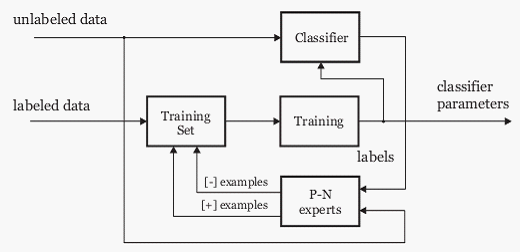
\includegraphics[width=\textwidth]{pn-learning}
	\caption{P-N learning示意图。}
	\label{fig:pn-learning}
\end{figure}

虽然P-expert和N-expert生成正负样本的过程本身也存在误差,但是
理论上的分析得出,只要P-expert和N-expert预测的准确率超过50\%就能够提高分类器的性能 \cite{p-n}。为了抑制``漂移''问题实现长时间目标跟踪,对在线分类器的``纠错''过程是必不可少。因此本文采用基于深度学习的目标检测模块作为P-expert和N-expert,经过大量离线样本的训练,该目标检测算法预测的正确率远远超过50\%,能够纠正在线学习所导致的漂移的问题。而且基于深度学习的检测模块与在线的分类器是相互独立的,不会形成在线式学习中出现的``正反馈''效应。

\section{目标检测辅助的Struck跟踪算法}
在第一帧的时候,使用目标检测算法自动搜索感兴趣目标,如果存在多个感兴趣目标需要手工选择具体的跟踪目标。一旦完成跟踪目标的选择,在线跟踪过程就开始了,跟踪算法分为三个模块:

跟踪模块。Struck跟踪算法从目标区域附近选取支持向量(即目标区域和容易被错分为目标的区域),选取的是特征是底层颜色直方图信息。支持向量的选取对Struck跟踪算法至关重要,跟踪过程中的``漂移''问题也是由于支持向量的集合中的正样本(跟踪器所认为的目标区域)偏离真实的目标区域所导致的。对$t+1$时刻的图像$x_{t+1}$,Struck跟踪算法利用更新后的模型在$t$时刻目标区域$y_t$的临域$R_{ts}=\left\{ {(u,v)|{u^2} + {v^2} < {r_s^2}}\right\}$内搜索目标。

检测模块。检测模块接受的输入为一张图像和跟踪模块在这一桢的跟踪结果$(x_t,y_t$。检测模块完成两项任务:1)验证区域$y_t$包含感兴趣目标的概率,如果低于某一阈值$\theta_p$,表示跟踪器在当前桢跟踪失败,如果连续$n$桢都跟踪失败,则需要重新初始化在线跟踪系统。2)如果区域$y_t$包含感兴趣目标的概率不低于$\theta_p$,则可以将区域$y_t$看作基于region proposal的深度学习算法中的一个proposal,检测算法不仅可以预测$y_t$包含目标的概率,还可以对$y_t$进行坐标回归得到$y_t'$。

P-N learning模块。基于在线学习的Struck跟踪模块会存在跟踪``漂移''问题,原因在于Struck跟踪模块会不可避免地引入错误的正支持向量,而引入错误正支持向量的原因在于Struck算法的分类模型进行了错误的分类。因此本文引入P-N learning模块来改进Struck的分类模型:1)对于跟踪结果$y_t$,检测模块的输出为$P(y_t)$表示区域$y_t$包含被跟踪目标的概率,$y_t'$表示对区域$y_t$的坐标回归。如果$P(y_t)<\theta_p$则认为当前桢跟踪失败,将支持模式$x_t$及其对应的支持向量移除,否则用$y_t^*=P(y_t)y_t + (1-P(y_t))y_t'$来代替$y_t$作为正支持向量,并对样本$(x_t,y_t^*)$做Struck算法中的ProcessOld模型更新操作。在Struck跟踪算法中选择负支持向量的方法为$y_-=\arg\min_{y \in Y} -\delta(y_t, y) - g(x_t, y)$,本文的方法中选择负支持向量的方法为$y_-=\arg\min_{y\in Y} -\delta(y_t,y) - P(y)$,其中$P(y)$是目标检测模块估计的区域$y$包含目标的概率。本文提出的基于region proposal的检测方法能够方便地估计各个区域包含目标的概率。基于深度学习的目标检测模块精度较高$P(y_t'\ \rm{contains\ object\ of\ interest})>0.5$,从理论上来讲P-N learning模块引入证样本$(x_t, y_t^*)$会改善Struck分类模型以实现对``漂移''的抑制。除此以外,更新后的正支持向量$y_t^*$也能够更新目标的大小,克服了Struck方法只能跟踪单一尺度目标的问题。


总结起来,本课题采用的跟踪方法采用P-N learning来融合基于在线学习的跟踪模块和基于离线知识的检测模块,以实现一种既能适应目标动态变化又能抑制``漂移''的跟踪效果。在实验过程中,前文所述的参数取值分别为跟踪搜索半径$r_s=30$,$r_d=50$,验证阈值$\theta_p=0.5$,$n=5$,将整个跟踪过程归纳于算法 \ref{al:track}。
\begin{algorithm}
	\caption{结合Struck目标跟踪和深度学习目标检测的长时间目标跟踪算法}
	\textbf{输入:}离线训练好的目标检测器$D$,初始桢$x_0$。\\
	\textbf{初始化:}使用目标检测器$D$在初始桢$x_0$上进行感兴趣目标的检测,如果存在多个感兴趣目标需要用户手工选择一个目标进行跟踪。目标在初始桢$x_0$中的区域为 $y_0$,对图像区域$y_0(x_0)$提取颜色直方图特征,并用来初始化Struck跟踪器。\\
	\textbf{For} $t=1,\cdots,T$ \textbf{do} \\
	(1)利用Struck跟踪器估计目标位置
		\[
		{y_t} = \arg \mathop {\max }\limits_{y \in {Y_t}} h(x_t^{{p_{t - 1}} \comp y})
		\]
	(2)使用$(x_t,y_t)$进行ProcessNew模型更新操作。\\
	(3)维护支持向量数目。\\
	\textbf{for} $j=1,\cdots,n_0$ \textbf{do}\\
	(4)\hspace{12pt}随机选择一个支持模式,并使用该支持模式进行ProcessOld模型更新操作。\\
	(5)\hspace{12pt}维护支持向量数目。\\
	\textbf{end}\\
	\textbf{if} $t\%3==0$ \textbf{do}\\
	(6)\hspace{12pt}目标检测器$D$验证区域$y_t$包含感兴趣目标的概率,如果不低于$\theta_p$转到(7),否则目标检测器认为当前桢目标已经跟丢了,如果连续$n$桢都跟丢,则重新初始化。\\
	(7)\hspace{12pt}使用检测器$D$在$y_t$的临域$R_{td}$内检测感兴趣目标,并选择于$y_t$重叠度最高的目标区域$y_t'$。将$(x_t,y_t')$做为样本进行ProcessNew更新并维护支持向量的数目。\\
	\textbf{end}\\
	\textbf{End}
	\label{al:track}
\end{algorithm}
\section{实验结果及分析}
本实验采用离线的方式处理图像序列旨在验证算法的有效性,为了模拟高精度目标检测算法通常不能实时运行的情况,如算法 \ref{al:track}所示实验过程中每3桢图像使用一次目标检测器。典型的图像序列跟踪效果如图 \ref{fig:track-result} 所示。
\begin{figure}[h]
	\subfigure[David]{
		\includegraphics[width=8cm, height=4cm]{david}
	}
	%\subfigure[Sylvester] {
	%	\includegraphics[width=8cm, height=4cm]{syl}
	%}
	\subfigure[Woman] {
		\includegraphics[width=8cm, height=4cm]{woman}
	}
	\subfigure[Car] {
		\includegraphics[width=8cm, height=4cm]{car}
	}
	\subfigure[Girl] {
		\includegraphics[width=8cm, height=4cm]{girl}
	}
	\subfigure[Faceocc] {
		\includegraphics[width=8cm, height=4cm]{faceocc}
	}
	\caption{在典型图像序列上的跟踪效果}
	\label{fig:track-result}
\end{figure}

本章所提出的融合离线和在线信息的跟踪算法目的在于实现长时间的目标跟踪。为了评估跟踪算法对时间的鲁棒性,本文采用Wu等 \cite{benchmark}提出的评估框架以及benchmark来评估本文提出的跟踪算法。中心误差是跟踪精度一种常用的度量方式,所谓中心误差是指跟踪到的目标对象的中心和ground truth的中心之间的欧式距离。图像序列中所有帧的平均中心误差可以用来度量该图像序列的整体跟踪效果。然而当跟踪失败之后,跟踪结果有可能是随机的,平均误差就不能正确地评估跟踪效果。因此,在中心误差的基础上,Wu等采用成功率图(success plot)来度量跟踪效果。每一帧的跟踪结果与ground truth之间的重叠度用Iou来度量,如果IoU高于某一阈值则认为跟踪成功。成功率图(success plot)显示的是当阈值从0变化到1时跟踪成功的图像帧的百分比。本文使用成功率图(success plot)下的面积(AUC)作为评估的量化指标。对时间鲁棒性的评估过程为,从不同的图像桢开始跟踪图像序列,以评估图像序列长度对跟踪算法的影响。图 \ref{fig:tre}显示了本文提出的跟踪算法和当前流行的跟踪算法的时间鲁棒性评估结果。
\begin{figure}
	\centering
	\includegraphics[scale=1]{tre}
	\caption{时间鲁棒性评估(TRE)结果。}
	\label{fig:tre}
\end{figure}

本章采用离线-在线的方式实现了一种长时间目标跟踪算法。离线的先验知识来源于基于region proposal的深度学习目标检测算法,在线式的跟踪算法采用的是Struck目标跟踪算法,作为先验知识的目标检测器以P-expert和N-expert的形式存在,采用P-N learning的方式将离线知识和在线分类器无缝结合起来,并且了克服Struck算法只能跟踪单一尺度目标的问题。